\documentclass[number, 3p, 10pt, times]{elsarticle}
\usepackage[position=top]{subfig}
\usepackage{amssymb}
\usepackage{amsmath}
\usepackage{amsthm}
\usepackage{rotating}
\usepackage{siunitx}
\usepackage{booktabs}
\usepackage{multicol}
\usepackage{multirow, bigdelim}
\usepackage{bm}
\usepackage{lineno}
\usepackage{framed}
\usepackage{algorithm}
\usepackage{algpseudocode}
\usepackage{verbatim}
\usepackage{colortbl}
\usepackage{url}
\usepackage{array}
\usepackage{setspace}
\usepackage{dcolumn}
\usepackage{nomencl} % Nomenclature package
\usepackage[T1]{fontenc}
\usepackage{tikz}
\usepackage{mathtools, cuted}
\usepackage[official]{eurosym}
\usepackage{pifont}% http://ctan.org/pkg/pifont
\newcommand{\cmark}{\ding{51}}%
\newcommand{\xmark}{\ding{55}}%
\usetikzlibrary{shapes, arrows, trees, positioning, fit, shadows, patterns, intersections, decorations.pathmorphing, decorations.pathreplacing}
\tikzset{
   brace_top/.style={
     decoration={brace},
     decorate
   },
   brace_bottom/.style={
     decoration={brace, mirror},
     decorate
   }
}
\makenomenclature
\setlength{\nomitemsep}{-\parskip} % Baseline skip between items
\renewcommand*\nompreamble{\begin{multicols}{2}}
\renewcommand*\nompostamble{\end{multicols}}
\newcommand\floor[1]{\lfloor#1\rfloor}
\newcommand\ceil[1]{\lceil#1\rceil}
\DeclareMathOperator*{\argmin}{\arg\!\min}
%\DeclarePairedDelimiter{\ceil}{\lceil}{\rceil}

\doublespacing

\newcommand\blfootnote[1]{%
  \begingroup
  \renewcommand\thefootnote{}\footnote{#1}%
  \addtocounter{footnote}{-1}%
  \endgroup
}
  
  
\journal{Solar Energy}

\begin{document}
\linenumbers

\begin{frontmatter}

\title{Evaluating zero-shot representation for univariate solar forecasting using foundation models}
% \title{Can zero-shot representation leap the persistence hurdle? Evaluating univariate solar irradiance forecasting in the era of foundation models}
\author[label1,label2]{Dazhi~Yang\corref{cor1}}
\address[label1]{School of Electrical Engineering and Automation, Harbin Institute of Technology, Harbin, Heilongjiang, China}
\cortext[cor1]{Corresponding author. }
\address[label2]{Key Laboratory of Energy Meteorology, China Meteorological Administration, Beijing, China}
\ead{yangdazhi.nus@gmail.com}


\begin{abstract}
Univariate solar forecasting remains a critical yet formidable challenge for solar grid integration, particularly for photovoltaic systems that either lack the data required for accurate physical modeling or have heterogeneous design parameters. Despite extensive research, eliminating the phase lag between forecasts and observations---often called the ``persistence hurdle''---remains difficult. Accordingly, I investigate a paradigm shift in the field: the transition from traditional regression-based forecasting to zero-shot representation learning via time series foundation models (TSFMs). Using a rigorous experimental framework across seven geographically diverse sites, I evaluate state-of-the-art TSFMs (released in 2024--2025) against established supervised baselines. The results reveal a pronounced ``efficiency gap'': most TSFMs fail to overcome the persistence-induced phase lag, and several yield negative forecast skill relative to the reference. In contrast, TabPFN---a tabular prior-data-fitted network---demonstrates superior utility, achieving a consistent 5\% forecast skill for both global and beam irradiance. These findings suggest that, for high-frequency stochastic solar transients, the structural priors of regression-based foundation models are more effective than the general-purpose sequence representations of current large-scale TSFMs. This work provides a new benchmark for univariate solar forecasting and offers a cautionary perspective on the zero-shot applicability of LLM-based forecasting models in highly variable physical systems. Data and code are released for reproducibility.


\textbf{Highlights}
\begin{itemize}
\item First systematic evaluation of foundation models for univariate solar forecasting
\item TSFMs fail to overcome the persistence hurdle and exhibit an efficiency gap
\item Regression-based TabPFN achieves 5\% forecast skill for GHI and BNI
\item Zero-shot representation is currently less robust than structured regression
\end{itemize}
\end{abstract}

\begin{keyword}
Solar forecasting \sep Zero-shot forecasting \sep Foundation models \sep Persistence hurdle\\
% \medskip
% \emph{Word count}: 5894.
\end{keyword}


\end{frontmatter}

\newpage 


\section{Introduction}\label{sec:intro}

Solar forecasting is conventionally categorized into three operational horizons: day-ahead (0--72 h), intra-day (0--4 h), and intra-hour (0--15 min). For the intra-hour horizon, ground-based sky imagers have long been proposed as the primary physical support \citep{YangBook}; however, their practical value remains contested, as camera-augmented models frequently struggle to provide a significant improvement on forecast skill over na{\"i}ve reference models \citep{Nouri2025}, such as the convex combination of climatology and persistence (CLIPER) \citep{YANG2019981}. Recently, the emergence of time-series foundation models (TSFMs), such as Amazon's Chronos \citep{Ansari2024} or Google's TimesFM \citep{Das2024}, has introduced a new paradigm, promising zero-shot capabilities learned from massive, cross-domain datasets. While these models are surrounded by significant industry hype, their efficacy in handling the stochastic nature of solar irradiance is not yet established. Therefore, in this work, I attempt to determine whether the deep temporal representations of foundation models can finally shatter the ``persistence hurdle'' in intra-hour forecasting, or if they represent another layer of algorithmic complexity that fails to outperform the basic benchmarks. 

Beyond the limitations of the persistence hurdle, the practical deployment of camera-based forecasting systems is further hindered by the realities of real-world energy infrastructure. Most solar assets operate without dedicated sky-imaging hardware, and even where on-site irradiance sensors exist, they are frequently subject to poor maintenance, sensor drift, or intermittent telemetry \citep{NIE2023171, Lin2025}. Furthermore, traditional physical models struggle with ``opaque variables'' that cameras cannot easily parameterize: heterogeneous site layouts in hilly terrain, complex shading on distributed rooftops \citep{PIERRO20171026}, and human-intervened events such as active power curtailment or localized equipment malfunctions \citep{BIRD2016577}. In these ``noisy'' environments, the rigid geometric assumptions of sky-imaging systems often collapse. This necessitates a transition toward univariate foundation models capable of identifying deep, latent signatures of system behavior directly from historical power data, offering a resilient forecasting solution that remains agnostic to site-specific physical complexities and sensor degradation.

The appeal of univariate solar forecasting has persisted from the earliest autoregressive models \citep{REIKARD2009342} and shallow neural networks \citep{PEDRO20122017} to contemporary deep learning architectures. Despite the rise of complex multi-modal systems, researchers remain focused on univariate approaches using long short-term memory (LSTM) \citep{DIAZBEDOYA2023117618} or convolutional neural networks (CNN) \citep{AITMANSOUR2024101886} due to their scenario-independence and minimal overhead. Within the machine learning landscape, a consensus has emerged that tree-based ensembles, such as extreme gradient boosting (XGBoost), often provide superior performance for tabularized time-series features due to their ability to handle nonlinearities and local variance without extensive hyperparameter tuning \citep{YAGLI2019487}. Similarly, LSTMs have been favored for their capacity to capture long-range temporal dependencies through gated architectures. However, a fundamental limitation persists: All traditional machine learning and deep learning models are data-hungry, requiring extensive site-specific historical training periods to achieve operational accuracy. This ``cold start'' requirement poses a significant barrier for newly commissioned solar sites where historical data is nonexistent. This critical gap highlights the ``zero-shot'' advantage of foundation models, which can theoretically provide good forecasts from the first moment of operation.

At a fundamental level, the distinction between traditional machine learning and foundation models lies in the transition from direct regression---mapping inputs to specific values---to representation-based inference, where forecasting is performed within a learned, universal latent space. Traditional univariate models operate through local pattern matching. These models attempt to minimize an objective function by mapping specific historical observations and engineered features directly to future values, effectively ``fitting'' the statistical noise and sensor bias of a single geographic location. Consequently, their predictive power is tethered to the stationarity of the local data distribution. In contrast, TSFMs leverage zero-shot representation learning derived from billions of diverse tokens \citep{Ansari2024, Das2024}. By pre-training on a massive corpus of cross-domain sequences \citep{Goswami2024}, models like Chronos do not merely regress a line; they identify the universal ``grammar'' of time---such as seasonality, trend-reversal, or stochastic volatility. For solar forecasting, this means the model can potentially interpret an irradiance ``ramp'' not as a unique local event, but as a specific temporal primitive it has encountered across a thousand different domains, allowing for a level of generalization that traditional regression models cannot achieve. 

To further refine the distinction between traditional and generative approaches, one must consider the emergence of prior-data fitted networks, such as TabPFN \citep{Hollmann2025}. While traditional models like XGBoost rely on iterative optimization to minimize local error \citep{Chen2016}, and TSFMs like Chronos leverage global temporal grammars \citep{Ansari2024}, TabPFN introduces a third mechanism: in-context Bayesian inference \citep{muller2024}. By approximating a posterior predictive distribution learned from millions of synthetic datasets during its own pre-training, TabPFN treats a small window of local historical data not as a training set, but as a contextual prompt \citep{Hollmann2025}. This allows it to compete with the zero-shot efficiency of TSFMs while maintaining the structured, feature-based rigor of tabular regression. Testing TabPFN alongside TSFMs allows us to distinguish whether the forecasting breakthrough stems from temporal sequence modeling (e.g., Chronos) or from the superior handling of small-sample tabular nonlinearities. 

Also standing between the site-specific optimization of traditional machine learning and the massive-scale pre-training of TSFMs is TiRex (Time-series Rex) \citep{Auer2025}, a model built upon the extended LSTM (xLSTM) architecture \citep{Beck2024}. While traditional LSTMs have long been favored for solar applications, they often suffer from memory saturation and an inability to revise past storage states when encountering abrupt atmospheric changes. TiRex addresses these shortcomings by incorporating exponential gating and a matrix memory structure, effectively modernizing the recurrent paradigm to compete with transformer-based attention mechanisms. In the context of this study, TiRex represents a ``special'' middle ground: It possesses the refined architectural inductive bias required to process high-frequency temporal sequences without the massive parameter overhead or tokenization requirements of models like Chronos or TimesFM. By considering TiRex, we can determine whether the intra-hour forecasting breakthrough necessitates the ``big data'' approach of generative pre-training or if superior recurrent architectural designs can sufficiently capture the stochastic volatility of solar irradiance. In summary, Table~\ref{tb:summary} summarizes the taxonomy of data-driven paradigms for time-series forecasting. 

\begin{table}[ht]
\centering
\caption{Taxonomy of data-driven paradigms for time series forecasting.}
\label{tb:summary}
\footnotesize
\begin{tabular}{@{}llll@{}}
\toprule
\textbf{Modeling paradigm} & \textbf{Representative} & \textbf{Core mechanism} & \textbf{Training requirement} \\ \midrule
Tabular regression & XGBoost & Gradient boosting & Extensive local history \\
Recurrent neural network regression & LSTM & Gated backpropagation & Extensive local history \\
Tabular foundation model & TabPFN & In-context Bayesian inference & Pre-trained (Zero-shot) \\
Recurrent foundation model & TiRex & xLSTM state-tracking & Pre-trained (Zero-shot) \\
Time series foundation model & Chronos & Transformer / tokenization & Pre-trained (Zero-shot) \\ \bottomrule
\end{tabular}
\end{table}

To evaluate the potential of zero-shot solar forecasting, I compare a range of modeling paradigms across seven geographically diverse sites. CLIPER is used as the standard reference, establishing a baseline for evaluating the forecast skill of other models. XGBoost, which typifies traditional machine learning, is compared against several state-of-the-art zero-shot TSFMs, including variants of Chronos \citep{Ansari2024}, TimesFM 2.5 \citep{Das2024}, and TinyTimeMixer (TTM) \citep{Ekambaram2024}. I further explore two specialized architectures, namely, the tabular meta-learning model TabPFN \citep{Hollmann2025} and the xLSTM-based TiRex \citep{Auer2025}. By assessing these recent forecasting models without site-specific training, I investigate whether large-scale pre-training can overcome data-scarcity and high-variability challenges in solar irradiance forecasting, thereby surmounting the persistence hurdle. 


\section{Data quality control and preprocessing}
The dataset used in this study integrates ground-based observations over a two-year period spanning 2023 and 2024 from the Surface Radiation Budget Network (SURFRAD) \citep{Augustine2000} with satellite-derived data from the latest version of the National Solar Radiation Database (NSRDB) \citep{XIE2023112195}. All seven SURFRAD stations are herein considered, and their metadata are listed in Table~\ref{tb:meta}. Given that foundation models for time-series forecasting are sensitive to outliers and gaps, I implement a multi-stage data processing pipeline consisting of rigorous quality control (QC) based on the Baseline Surface Radiation Network (BSRN) standards \citep{Forstinger2021}, temporal aggregation, and data filling. 

\begin{table}[ht]
\centering
\caption{SURFRAD station metadata. The missing percentage is computed for 2023 and 2024.}
\label{tb:meta}
\footnotesize
\begin{tabular}{lccccccc}
\toprule
Station & BON & DRA & FPK & GWN & PSU & SXF & TBL \\
\midrule
Latitude ($^\circ$) & 40.05 & 36.62 & 48.31 & 34.25 & 40.72 & 43.73 & 40.12 \\
Longitude ($^\circ$) & $-$88.37 & $-$116.02 & $-$105.10 & $-$89.87 & $-$77.93 & $-$96.62 & $-$105.24 \\
Elevation (m) & 230 & 1007 & 634 & 98 & 376 & 473 & 1689 \\
Missing (\%) & 9.1 & 3.8 & 5.9 & 6.7 & 4.3 & 5.9 & 4.8 \\
\bottomrule
\end{tabular}
\end{table}

\subsection{Quality control sequence}
The raw 1-min SURFRAD measurements for global horizontal ($G_h$), beam normal ($B_n$), and diffuse horizontal ($D_h$) irradiance are subjected to a three-tier QC procedure. The first tier identifies physical outliers by ensuring the components do not exceed upper limits defined by the extraterrestrial irradiance ($E_0$) and the solar zenith angle ($Z$); this is known as the extremely rare limits (ERL) test:
\begin{align}
    -2 < G_h & \leq 1.2 E_0 \cos^{1.2}Z + 50, \\
    -2 < B_n & \leq 0.95 E_0 \cos^{0.2}Z + 10, \\
    -2 < D_h & \leq 0.75 E_0 \cos^{1.2}Z + 30.
\end{align}

The second tier verifies the consistency of the three components. For periods where $G_h > 50$ W/m$^2$, the test evaluates the relative difference between measured $G_h$ and the value calculated from its components ($B_n \cos Z + D_h$), and data points are rejected if they fail the following criteria:
\begin{equation}
    \left| \frac{G_h - (B_n \cos Z + D_h)}{G_h} \right| \leq 
    \begin{cases} 
    0.08 & \text{if } Z < 75^\circ \\
    0.15 & \text{if } 75^\circ \leq Z < 93^\circ
    \end{cases}.
\end{equation}
This test is known as the BSRN's closure test.

The third tier utilizes dimensionless transmittances, i.e., the $k$-indices, to detect unphysical atmospheric conditions. Let $k_t = G_h / (E_0 \cos Z)$ be the clearness index, $k_b = B_n / E_0$ be the beam transmittance, and $k = D_h / G_h$ be the diffuse fraction. A measurement is considered valid only if it passes all the following filters:
\begin{align}
    k_b &< k_t \quad \text{for } G_h > 50\text{ W/m}^2, \\
    k_b &< \frac{1100 + 0.03h}{E_0} \quad \text{where } h = \text{elevation in meters}, \\
    k_t &< 1.35 \quad \text{for } G_h > 50\text{ W/m}^2, \\
    k &< 
    \begin{cases} 
    1.05 & \text{for } Z < 75^\circ \text{ and } G_h > 50\text{ W/m}^2\\
    1.10 & \text{for } Z \geq 75^\circ \text{ and } G_h > 50\text{ W/m}^2
    \end{cases}, \\
    k &< 0.96 \quad \text{for } k_t > 0.6, Z < 85^\circ, \text{ and } G_h > 150\text{ W/m}^2.
\end{align}

\subsection{Data aggregation and filling}
To align the data for intra-hour forecasting, the post-QC 1-min samples are resampled to a 15-min resolution using the interval endpoint as the label, i.e., a right-aggregation scheme. An interval is valid only if it contains $\geq 7$ successful 1-min observations; otherwise, it is marked as missing.

To ensure a continuous time series for the foundation models, missing SURFRAD observations are filled using 5-min NSRDB data \citep{Yang2021NSRDB} resampled to the same 15-min temporal grid. Finally, to eliminate nighttime noise, all irradiance values are set to zero when the zenith angle $Z > 90^\circ$. The resulting dataset provides a synchronized time series of measured, modeled, and clear-sky irradiance components. It should be noted that the clear-sky irradiance in NSRDB is computed via the REST2 model \citep{GUEYMARD2008272}, powered by the Modern-Era Retrospective Analysis for Research and Applications, version 2 \citep{Gelaro2017}.

\section{Models and implementation}
In this work, a diverse suite of forecasting approaches is evaluated to benchmark the current state of zero-shot solar irradiance forecasting across varying climates. The CLIPER model \citep{YANG2019981} is used as the fundamental reference, establishing the performance floor expected from other forecasting models. To represent established machine learning practices, XGBoost \citep{Chen2016}, a widely adopted gradient-boosted decision tree framework, is used. The core of the current investigation, however, focuses on the emerging class of zero-shot TSFMs. This includes large-scale pre-trained architectures designed for cross-domain generalization, namely, Amazon's Chronos (in both its standard v2 and optimized ``Bolt'' variants) \citep{Ansari2024}, Google's TimesFM 2.5 \citep{Das2024}, and IBM's TinyTimeMixer (TTM) series \citep{Ekambaram2024}. Furthermore, I include two specialized zero-shot models that leverage unique architectural priors: TabPFN \citep{Hollmann2025}, a prior-data-fitted network \citep{muller2024} that treats forecasting as a tabular in-context learning task, and TiRex \citep{Auer2025}, a foundation model built on the recently introduced xLSTM architecture \citep{Beck2024}. By categorizing these models into baselines, traditional ML, and zero-shot foundation models, this work aims to provide a comprehensive assessment of their ability to handle solar variability without the need for site-specific fine-tuning. It should be noted that all models, besides CLIPER and XGBoost, are exceedingly recent; thus, the results herein represent the state of the art in zero-shot solar forecasting.

All computer experiments conducted here were executed using a late 2024 MacBook Pro equipped with the Apple M4 Max chip. This hardware configuration features a 16-core CPU and a 40-core GPU, supported by 128 GB of unified memory with a bandwidth of up to 546 GB/s. The primary advantage of this architecture for solar forecasting research is its unified memory architecture, which allows the GPU to directly access the entire 128 GB memory pool. This eliminates the data-transfer bottlenecks typically found in traditional discrete GPU setups, facilitating the efficient handling of the large-scale datasets and complex time-series foundation models used in this study.

\subsection{CLIPER}
Unlike a simple persistence model that assumes the atmospheric state remains constant over the forecast horizon, CLIPER utilizes an optimal linear combination of the most recent observation and the long-term historical average \citep{YANG2019981}. This approach provides a tighter ``no-skill'' baseline by accounting for both the short-term autocorrelation of the atmosphere and the underlying climatological distribution of solar resources. In this study, CLIPER is applied to the clear-sky index ($\kappa$) time series to decouple the stochastic atmospheric attenuation from the deterministic diurnal solar cycle. Mathematically, the forecast clear-sky index for the next time step, $\hat{\kappa}_{t+1}$, is formulated as:
\begin{equation}
    \hat{\kappa}_{t+1} = \gamma \kappa_{t} + (1 - \gamma) \bar{\kappa}
\end{equation}
where $\kappa_{t}$ represents the persistence component derived from the current observation, and $\bar{\kappa}$ is the climatological mean clear-sky index calculated from the training dataset. The weighting factor $\gamma$ is determined by the first-order autocorrelation of the clear-sky index series. The final irradiance forecast is subsequently reconstructed by modulating the forecast clear-sky index with the corresponding clear-sky irradiance. 

The implementation of CLIPER involved a rigorous calibration phase using data from the year 2023 to estimate the site-specific parameters $\bar{\kappa}$ and $\gamma$. To mitigate numerical instability and noise associated with low-sun angles, clear-sky indices were only computed for records where the solar zenith angle was less than 85$^\circ$, and the clear-sky irradiance exceeded 10~W/m$^2$. For the evaluation period in 2024, the model maintained temporal continuity by utilizing the final observations of 2023 to initialize the first forecasts of the test set. In instances where the persistence component was unavailable---such as during the first morning interval or following a data gap---the model defaulted to the climatological mean $\bar{\kappa}$. Finally, a post-processing filter was applied to set all nighttime forecasts ($Z> 90^\circ$) to zero and clip any non-physical negative values.

\subsection{XGBoost}
XGBoost is an ensemble method based on gradient-boosted decision trees that minimizes a regularized objective function, which includes a convex loss function and a penalty term for model complexity to prevent overfitting \citep{Chen2016}. The model iteratively adds weak learners to predict the residuals of previous trees, effectively mapping a high-dimensional feature vector $\mathbf{x}_t$ to the target variable. To preserve the cyclical nature of the solar time series, temporal indicators, such as the hour of the day or day of the year, are transformed into cyclic coordinates using sine and cosine functions, ensuring that the model recognizes the continuity between the end of one period and the start of the next.

The implementation utilizes a feature set $\mathbf{x}$ comprising the solar zenith angle, cyclic temporal coordinates, and autoregressive lags. Specifically, the input vector includes the four immediate preceding observations ($t-1$ to $t-4$) and a seasonal lag of 24 h ($t-96$ for the 15-min resolution) to provide the model with both recent trend and diurnal context. The ensemble was configured with 500 boosting rounds, a learning rate of 0.05, and a maximum tree depth of 6, with training restricted to daytime data ($Z< 85^\circ$) to avoid biasing the learners with nocturnal zeros. Early stopping with a patience of 50 rounds was applied against a 10\% sequential validation split of the 2023 training data. During inference on the 2024 test set, all outputs were clipped at zero and masked for nighttime periods ($Z> 90^\circ$) to ensure physical consistency.

\subsection{Chronos-Bolt and Chronos-2}
Chronos is a framework for pre-trained probabilistic time-series models that adapts the transformer-based language modeling paradigm to numerical sequences \citep{Ansari2024}. The model utilizes a tokenization pipeline consisting of mean scaling---where each sequence is normalized by the mean of its absolute values---and linear quantization into a discrete vocabulary of tokens. By treating forecasting as a representation task, Chronos leverages the cross-entropy loss function and the self-attention mechanisms of large language models (LLMs) to learn complex temporal dynamics from a massive corpus of diverse datasets, including synthetic series generated via Gaussian processes. Formally, for a given historical context $\mathbf{x}_{1:C}$, the model generates a probabilistic forecast by sampling multiple trajectories from the predicted categorical distribution:
\begin{equation}
    P(x_{C+1:C+h} | \mathbf{x}_{1:C}) = \prod_{i=1}^{h} P(x_{C+i} | \mathbf{x}_{1:C+i-1})
\end{equation}
where $h$ denotes the forecast horizon, indexed by $i$. In this work, I focus exclusively on 1-step-ahead forecasting ($h=1$) to evaluate the immediate predictive accuracy of the models. The resulting tokenized outputs are subsequently mapped back to real-valued irradiance or clear-sky index values through dequantization and inverse scaling, enabling robust zero-shot generalization to unseen datasets.

In this study, I evaluate two specific variants of the architecture: Chronos-Bolt and Chronos-2. The Chronos-Bolt variant is a high-throughput encoder--decoder model based on the T5 architecture that replaces autoregressive decoding with a direct multi-step forecasting head. It employs a patching mechanism to group historical observations into chunks, significantly reducing memory consumption and improving inference speed by up to 250 times compared to the original T5-based iterations. Conversely, Chronos-2 is a universal forecasting model that introduces a group attention mechanism to enable in-context learning across multiple related time series within a batch. Both models were implemented using a context length of 512 steps to capture sufficient historical trends, with inference performed at 15-min resolution. For each forecast step, the median value (50th percentile) was extracted from the sampled distribution as the point forecast. To maintain physical consistency, nighttime values were masked based on a solar zenith angle threshold ($Z > 90^\circ$), and all forecasts were clipped to ensure non-negativity.

\subsection{TimesFM-2.5}
The architecture of TimesFM utilizes a decoder-only transformer that operates on patched time-series data, where contiguous segments of the input sequence are mapped into high-dimensional tokens \citep{Das2024}. This patching mechanism enables the model to capture long-range dependencies while maintaining computational efficiency. TimesFM is pre-trained on a massive corpus of diverse datasets spanning billions of time points using a causal language modeling objective. During inference, the model produces a distribution of future values by processing a historical context and decoding the subsequent steps through a specialized quantile head, which ensures the probabilistic consistency of the outputs. For a given context length $C$, the forecast is generated as:
\begin{equation}
    \hat{x}_{C+1} = f_\text{dec}(f_\text{enc}(\mathbf{x}_{1:C}))
\end{equation}
where $f_\text{enc}$ represents the patch-based embedding encoder and $f_\text{dec}$ denotes the transformer decoder and prediction head. 

The implementation utilized the TimesFM-2.5-200m-pytorch variant, deployed on a Metal Performance Shaders (MPS) backend for accelerated inference. A significant historical context of 1024 steps was provided to the model to maximize its internal state representation of diurnal and synoptic patterns at 15-min resolution. To optimize throughput, the model's \texttt{compiled\_decode} method was used with a batch size of 1024, bypassing standard high-level wrappers. The forecasting configuration included input normalization, forced flip invariance, and a continuous quantile head to ensure non-negative and physically plausible predictions. For each 15-min interval in the 2024 test period, the median point forecast was extracted. Similar to the other models in this study, forecasts were only generated for daytime periods where the solar zenith angle was less than $90^\circ$, and all resulting values were post-processed with a non-negativity clip to maintain physical consistency.

\subsection{TTM-R1 and TTM-R2}
TTM represents a class of lightweight, non-transformer foundation models designed for high-efficiency time-series forecasting \citep{Ekambaram2024}. Unlike traditional transformer-based architectures that rely on computationally intensive self-attention mechanisms, TTM is built upon the TSMixer backbone, which utilizes a series of multilayer perceptron blocks to mix information across both the temporal and channel dimensions. To handle diverse temporal resolutions during pre-training, TTM introduces adaptive patching and resolution prefix tuning, allowing the model to condition its internal representations on the specific frequency of the input data. The model operates by projecting time-series patches into a latent space where temporal dependencies are captured through gated attention and simple perceptron blocks. This streamlined design allows TTM to achieve state-of-the-art zero-shot performance with fewer than one million parameters.

In this study, I consider two TTM variants, namely, TTM-R1 and TTM-R2. While both variants share the same underlying architecture, TTM-R1 was pretrained on a public dataset comprising approximately 250 million samples. In contrast, TTM-R2 was trained on a significantly larger corpus of approximately 700 million samples to enhance its generalization capabilities across diverse data distributions. Both models were implemented in a zero-shot configuration using a fixed context length of 512 steps to generate forecasts at a 15-min resolution. To maximize computational efficiency on the MPS backend, inference was performed in batches of 64. Although the models were configured with a default prediction length of 96, only the first step ($h=1$) was extracted for each rolling forecast window to maintain consistency with the 1-step-ahead forecasting framework. Final predictions were again post-processed to mask nighttime values.

\subsection{TabPFN-2.5}
TabPFN is a transformer-based foundation model designed for supervised learning on tabular data via in-context learning \citep{Hollmann2025}. Unlike conventional machine-learning models that require gradient-based optimization for each new task, TabPFN approximates Bayesian inference in a single forward pass by processing a labeled training context alongside test inputs. The model is pretrained on a massive corpus of diverse synthetic datasets generated from structural causal models, enabling it to generalize to unseen tabular structures without site-specific hyperparameter tuning. Formally, the model directly yields the posterior predictive distribution for a test input $\mathbf{x}_\text{test}$ given a training context $\mathcal{D} = \{(\mathbf{x}_i, y_i)\}_{i=1}^n$:
\begin{equation}
    p(y_\text{test} | \mathbf{x}_\text{test}, \mathcal{D}) = \text{Transformer}(\mathbf{x}_\text{test}, \mathcal{D})
\end{equation}
This architecture allows the model to handle nonlinear feature interactions and missing values natively, providing a robust zero-shot baseline for complex regression tasks.

In this study, the TabPFN-v2.5 Regressor is applied directly to a tabular feature matrix identical to that of the XGBoost baseline. The input vector $\mathbf{x}$ comprises the solar zenith angle, cyclic temporal coordinates (sine and cosine of the hour and day), and five autoregressive lags ($t-1$ to $t-4$ and $t-96$). The model was implemented using the \texttt{tabpfn-client} library to leverage cloud-based inference, with the training context $\mathcal{D}$ derived from daytime observations ($Z < 85^\circ$) in the 2023 dataset. It should be highlighted that, for the 2024 evaluation period, TabPFN generates all point forecasts in one go, which differs from the rolling forecasting employed by the TSFMs. 

\subsection{TiRex}
TiRex is a foundation model based on the xLSTM architecture, specifically designed to bridge the gap between traditional recurrent state-tracking and modern transformer-based in-context learning \citep{Auer2025}. Unlike the transformer models used in this study, which rely on global self-attention, TiRex utilizes xLSTM, which features exponential gating and a memory-augmented structure to maintain stable latent states over long sequences. This allows the model to approximate hidden system dynamics without the quadratic computational complexity of attention mechanisms. During training, the model is optimized using a contiguous patch masking strategy, which forces it to learn coherent multi-step dependencies by forecasting over contiguous missing segments. Formally, the model approximates the conditional distribution of future steps given a historical context $\mathbf{x}_{1:C}$ through a decoder-only recurrent mapping:
\begin{equation}
    P(x_{C+1:C+h} | \mathbf{x}_{1:C}) = \mathcal{F}_{\text{xLSTM}}(\mathbf{x}_{1:C})
\end{equation}
where $\mathcal{F}_{\text{xLSTM}}$ represents the stack of xLSTM blocks that propagate the hidden state and cell state to generate probabilistic forecasts across the specified horizon.

The implementation utilized the 35-million-parameter TiRex foundation model, which was loaded using the \texttt{tirex} library with a PyTorch backend for MPS acceleration. A context length of 1024 steps was selected to provide the recurrent cells with sufficient historical information to initialize their internal states at a 15-min resolution. To optimize inference, data was processed in batches of 64 using a sliding window approach, and mean estimates were extracted for each forecast point. Consistent with the previous models, only the first forecast step of each window was used for the rolling forecast comparison. 

\section{Results and discussion}
The evaluation procedure was conducted across all seven SURFRAD stations. For each station, the analysis utilized ground-truth data from the year 2024 to evaluate 1-step-ahead forecasts for both GHI and BNI. These variables were assessed under two primary modeling configurations: direct forecasting on the observation time series and a decomposition approach in which the model forecasts the clear-sky index, which is subsequently converted back to irradiance for evaluation; these two configurations are annotated as ``Direct'' and ``Kappa,'' respectively. To ensure a rigorous assessment of performance, quantitative metrics---including the root mean square error (RMSE), mean bias error (MBE), and their respective normalized percentages---were calculated exclusively for valid daytime periods, defined by a solar zenith angle threshold of $Z < 85^\circ$. Furthermore, a skill-score analysis was performed by comparing each model's RMSE against the performance of CLIPER, quantifying the percentage improvement over a standard reference. More specifically, the skill score is given by
\begin{equation}
\label{eq:ss1}
    s = \frac{\text{RMSE}_r - \text{RMSE}_f}{\text{RMSE}_r - \text{RMSE}_p},
\end{equation}
where $\text{RMSE}_f$, $\text{RMSE}_r$, and $\text{RMSE}_p$ are the RMSEs of a model of interest, the reference model, and the perfect model, respectively. By assuming $\text{RMSE}_p = 0$, Eq.~(\ref{eq:ss1}) reduces to $s = 1-\text{RMSE}_f/\text{RMSE}_r$. 

\subsection{Overall performance}
Tables~\ref{tb:RMSEGh} and \ref{tb:RMSEBn} present the RMSE for GHI and BNI forecasts across seven SURFRAD stations for the year 2024. The most prominent finding is that TabPFN-2.5-Kappa achieves the lowest RMSE in 13 out of 14 cases---covering all seven stations and both irradiance components---with the sole exception of the BNI forecast at the TBL station, where TabPFN-2.5-Direct slightly outperforms it. While certain architectures excel, the performance across the foundation model category is surprisingly heterogeneous. Among these, TiRex-Direct and TimesFM-2.5-Kappa offer the most competitive results, often matching or exceeding the XGBoost-Direct baseline. In contrast, the four Chronos variants, despite their demonstrated success in broader time-series benchmarks, perform poorly here; this is likely because their zero-shot categorical distribution modeling struggles with the high-frequency stochasticity and sharp gradients inherent to 15-min solar irradiance data. Finally, the TTM variants exhibit limited performance as well, potentially due to their lightweight MLP-Mixer architecture, which, while computationally efficient, may lack the expressive capacity required to capture complex atmospheric transients compared to the larger transformer-based or xLSTM-based counterparts.

\begin{table}[!ht]
\centering
\caption{Evaluation of the GHI forecasting performance across seven SURFRAD stations for the year 2024. Values represent the RMSE in W/m$^2$, with its normalized version (nRMSE, \%) provided in parentheses. The best performing model for each station is in bold.}
\label{tb:RMSEGh}
\footnotesize
\begin{tabular}{lrrrrrrrr}
\toprule
 & BON & DRA & FPK & GWN & PSU & SXF & TBL & Average \\
\midrule
CLIPER & 73.0 (19.1) & 59.2 (11.5) & 73.5 (20.5) & 81.3 (20.2) & 87.3 (25.0) & 71.2 (19.5) & 92.6 (21.8) & 77.6 (19.4) \\
XGBoost-Direct & 73.5 (19.2) & 58.5 (11.4) & 72.7 (20.2) & 79.3 (19.7) & 85.3 (24.4) & 70.2 (19.3) & 93.1 (21.9) & 76.8 (19.2) \\
XGBoost-Kappa & 70.8 (18.5) & 56.9 (11.0) & 71.3 (19.9) & 77.8 (19.3) & 84.4 (24.1) & 68.9 (18.9) & 90.5 (21.3) & 75.1 (18.8) \\
Chronos-Bolt-Direct & 75.2 (19.6) & 62.4 (12.1) & 75.3 (21.0) & 82.8 (20.6) & 88.2 (25.2) & 73.3 (20.1) & 96.9 (22.8) & 79.9 (20.0) \\
Chronos-Bolt-Kappa & 72.9 (19.1) & 59.9 (11.6) & 73.7 (20.5) & 80.8 (20.1) & 86.4 (24.7) & 71.4 (19.6) & 94.4 (22.2) & 77.8 (19.5) \\
Chronos-2-Direct & 73.9 (19.3) & 62.1 (12.1) & 75.2 (20.9) & 81.2 (20.2) & 87.1 (24.9) & 72.7 (20.0) & 96.9 (22.8) & 79.1 (19.8) \\
Chronos-2-Kappa & 73.8 (19.3) & 62.0 (12.0) & 75.8 (21.1) & 81.0 (20.1) & 87.8 (25.1) & 73.5 (20.2) & 97.9 (23.1) & 79.6 (19.9) \\
TimesFM-2.5-Direct & 72.2 (18.9) & 59.2 (11.5) & 73.1 (20.4) & 80.1 (19.9) & 85.2 (24.4) & 70.6 (19.4) & 94.4 (22.2) & 77.1 (19.3) \\
TimesFM-2.5-Kappa & 71.8 (18.8) & 59.1 (11.5) & 73.0 (20.3) & 79.4 (19.7) & 85.2 (24.4) & 70.5 (19.4) & 93.3 (22.0) & 76.7 (19.2) \\
TTM-R1-Direct & 76.2 (19.9) & 63.0 (12.2) & 76.1 (21.2) & 84.6 (21.0) & 88.7 (25.4) & 74.6 (20.5) & 95.4 (22.5) & 80.4 (20.1) \\
TTM-R1-Kappa & 79.1 (20.7) & 66.4 (12.9) & 76.7 (21.4) & 83.7 (20.8) & 89.7 (25.7) & 76.7 (21.0) & 97.9 (23.1) & 82.0 (20.5) \\
TTM-R2-Direct & 78.4 (20.5) & 67.7 (13.1) & 77.1 (21.5) & 86.6 (21.5) & 90.0 (25.7) & 75.9 (20.8) & 97.6 (23.0) & 82.4 (20.6) \\
TTM-R2-Kappa & 78.5 (20.5) & 66.0 (12.8) & 76.2 (21.2) & 82.8 (20.6) & 89.2 (25.5) & 76.1 (20.9) & 98.2 (23.1) & 81.6 (20.4) \\
TabPFN-2.5-Direct & 70.6 (18.4) & 56.9 (11.1) & 71.3 (19.8) & 77.6 (19.3) & 82.9 (23.7) & 68.3 (18.7) & 90.5 (21.3) & 74.7 (18.7) \\
TabPFN-2.5-Kappa & \textbf{69.6 (18.2)} & \textbf{56.2 (10.9)} & \textbf{70.4 (19.6)} & \textbf{76.3 (18.9)} & \textbf{82.1 (23.5)} & \textbf{67.5 (18.5)} & \textbf{89.4 (21.1)} & \textbf{73.8 (18.4)} \\
TiRex-Direct & 71.8 (18.8) & 59.0 (11.5) & 72.4 (20.2) & 79.0 (19.6) & 85.1 (24.3) & 70.2 (19.3) & 92.8 (21.9) & 76.5 (19.1) \\
TiRex-Kappa & 76.2 (19.9) & 64.5 (12.5) & 75.0 (20.9) & 80.3 (19.9) & 88.5 (25.3) & 74.0 (20.3) & 97.1 (22.9) & 80.0 (20.0) \\
\bottomrule
\end{tabular}
\end{table}

\begin{table}[!ht]
\centering
\caption{Same as Table~\ref{tb:RMSEGh}, but for BNI.}
\label{tb:RMSEBn}
\footnotesize
\begin{tabular}{lrrrrrrrr}
\toprule
 & BON & DRA & FPK & GWN & PSU & SXF & TBL & Average \\
\midrule
CLIPER & 122.7 (30.8) & 110.7 (16.0) & 129.5 (31.3) & 117.1 (28.1) & 132.1 (38.6) & 121.4 (30.0) & 153.0 (29.8) & 127.2 (28.0) \\
XGBoost-Direct & 119.4 (29.9) & 107.5 (15.6) & 126.3 (30.5) & 113.7 (27.3) & 128.8 (37.5) & 118.1 (29.1) & 148.1 (28.8) & 123.7 (27.2) \\
XGBoost-Kappa & 118.9 (29.9) & 106.6 (15.4) & 126.2 (30.5) & 112.7 (27.0) & 128.4 (37.5) & 117.0 (28.9) & 147.6 (28.8) & 123.1 (27.1) \\
Chronos-Bolt-Direct & 125.7 (31.5) & 114.8 (16.6) & 132.5 (32.1) & 120.3 (28.9) & 135.4 (39.5) & 125.3 (30.9) & 156.7 (30.5) & 130.7 (28.7) \\
Chronos-Bolt-Kappa & 124.4 (31.3) & 112.6 (16.3) & 131.4 (31.8) & 118.4 (28.4) & 134.1 (39.1) & 124.1 (30.7) & 155.0 (30.2) & 129.2 (28.4) \\
Chronos-2-Direct & 131.2 (32.9) & 120.5 (17.4) & 140.6 (34.0) & 124.5 (29.9) & 140.5 (40.9) & 131.2 (32.3) & 169.1 (32.9) & 137.6 (30.2) \\
Chronos-2-Kappa & 131.8 (33.1) & 120.6 (17.4) & 142.1 (34.4) & 125.6 (30.1) & 141.2 (41.2) & 131.8 (32.6) & 168.4 (32.8) & 138.1 (30.4) \\
TimesFM-2.5-Direct & 121.0 (30.3) & 110.5 (16.0) & 127.6 (30.9) & 114.6 (27.5) & 130.7 (38.1) & 119.9 (29.5) & 151.0 (29.4) & 125.6 (27.6) \\
TimesFM-2.5-Kappa & 121.0 (30.4) & 109.5 (15.8) & 127.4 (30.8) & 114.6 (27.5) & 130.7 (38.1) & 119.7 (29.6) & 151.2 (29.5) & 125.5 (27.6) \\
TTM-R1-Direct & 124.6 (31.2) & 115.4 (16.7) & 132.2 (32.0) & 119.4 (28.7) & 133.4 (38.9) & 123.9 (30.5) & 154.8 (30.1) & 129.6 (28.5) \\
TTM-R1-Kappa & 133.2 (33.4) & 122.1 (17.7) & 134.5 (32.5) & 120.2 (28.9) & 137.2 (40.0) & 131.4 (32.4) & 163.3 (31.8) & 135.2 (29.7) \\
TTM-R2-Direct & 124.8 (31.3) & 115.3 (16.7) & 131.5 (31.8) & 119.4 (28.7) & 133.2 (38.8) & 124.3 (30.6) & 155.5 (30.3) & 129.7 (28.5) \\
TTM-R2-Kappa & 131.8 (33.0) & 120.0 (17.4) & 133.7 (32.3) & 117.9 (28.3) & 135.7 (39.5) & 130.6 (32.2) & 162.5 (31.6) & 133.8 (29.4) \\
TabPFN-2.5-Direct & 117.5 (29.5) & 105.6 (15.3) & 124.2 (30.0) & 110.9 (26.6) & 126.0 (36.7) & 116.2 (28.6) & \textbf{145.2 (28.3)} & 121.4 (26.7) \\
TabPFN-2.5-Kappa & \textbf{117.1 (29.4)} & \textbf{104.6 (15.1)} & \textbf{123.7 (29.9)} & \textbf{110.6 (26.5)} & \textbf{125.2 (36.5)} & \textbf{115.6 (28.6)} & 145.4 (28.4) & \textbf{120.9 (26.6)} \\
TiRex-Direct & 121.9 (30.6) & 109.8 (15.9) & 128.9 (31.2) & 115.2 (27.7) & 132.3 (38.6) & 121.0 (29.8) & 153.9 (30.0) & 126.8 (27.9) \\
TiRex-Kappa & 129.4 (32.4) & 114.9 (16.6) & 131.9 (31.9) & 115.8 (27.8) & 135.2 (39.4) & 127.2 (31.4) & 161.2 (31.4) & 131.6 (28.9) \\
\bottomrule
\end{tabular}
\end{table}

Tables~\ref{tb:RMSEGh} and \ref{tb:RMSEBn} also demonstrate that for about half of the architectures, including XGBoost, Chronos, TimesFM, and TabPFN, the Kappa configuration---forecasting $\kappa$ followed by irradiance reconstruction---yields lower RMSE values than direct forecasting. This empirical evidence validates the methodology of decoupling the deterministic, double-seasonal component of solar irradiance from stochastic cloud attenuation, aligning with established theoretical frameworks in the field \citep{YangBook}. Surprisingly, this trend does not hold for models such as TTM or TiRex. One potential explanation for this discrepancy is the utilization of extensive historical contexts ($C=512$ or $1024$), where the inclusion of long sequences of zero values during nocturnal periods may degrade the model's internal representation of the $\kappa$ series. Because $\kappa$ is mathematically undefined or highly volatile at very low irradiance levels, these models may struggle to distinguish between physical atmospheric clearing and numerical noise within the context window, whereas direct forecasting allows the model to leverage the simpler, clear-sky-dominated signal of the diurnal cycle.

Across all models, the DRA station consistently exhibits the lowest RMSE and nRMSE values, with TabPFN-2.5-Kappa achieving 56.2 W/m$^2$ for GHI and 104.6 W/m$^2$ for BNI. This superior performance is primarily attributed to the station's location in an arid environment, where frequent clear-sky conditions result in a deterministic signal that is more easily captured by the models' internal representations. Conversely, the PSU station consistently yields the highest errors across all evaluation metrics. This reflects the significant challenges posed by more complex and volatile atmospheric regimes; as noted by \citet{YANG2022743}, the PSU station's proximity to Pittsburgh, Pennsylvania---one of the cloudiest cities in the United States---results in a high frequency of intermediate and overcast conditions. Such conditions increase the difficulty of forecasting, as rapid fluctuations in cloud optical depth create stochastic transients that univariate models cannot anticipate without exogenous spatial data.

Given that the mean square error can be decomposed into a variance and a bias term, it is of interest to examine the MBE. Table~\ref{tb:MBEGh} and \ref{tb:MBEBn} show the MBE results of various models at seven SURFRAD stations. For GHI forecasts, the bias remains notably low for the majority of the models, with the TabPFN-2.5-Direct variant achieving the lowest average absolute MBE of 0.5 W/m$^2$ (0.1\%). Chronos-Bolt-Kappa also exhibits exceptional bias characteristics at several stations, notably achieving a near-zero bias (0.0\%) at the GWN, PSU, and SXF stations. In contrast, certain zero-shot models such as TTM-R2-Direct show a systematic over-forecasting trend, with a significant average nMBE of 5.7\%. This suggests that while representation learning can capture temporal patterns, architectural choices like the MLP-Mixer in TTM can occasionally lead to unscaled biases compared to transformer-based counterparts.

\begin{table}[!ht]
\centering
\caption{Mean bias error (MBE), in W/m$^2$, and normalized MBE, in \%, of the GHI forecasts. The best performing model for each station is in bold.}
\label{tb:MBEGh}
\footnotesize
\begin{tabular}{lrrrrrrrr}
\toprule
 & BON & DRA & FPK & GWN & PSU & SXF & TBL & Average \\
\midrule
CLIPER & $-$2.8 ($-$0.7) & $-$3.3 ($-$0.6) & \textbf{$-$0.2 ($-$0.1)} & $-$2.6 ($-$0.6) & $-$3.5 ($-$1.0) & $-$0.3 ($-$0.1) & $-$1.8 ($-$0.4) & $-$2.1 ($-$0.5) \\
XGBoost-Direct & $-$2.8 ($-$0.7) & 1.2 (0.2) & 1.0 (0.3) & $-$1.6 ($-$0.4) & $-$2.9 ($-$0.8) & 0.6 (0.2) & $-$0.7 ($-$0.2) & $-$0.8 ($-$0.2) \\
XGBoost-Kappa & $-$2.8 ($-$0.7) & $-$0.8 ($-$0.2) & 2.1 (0.6) & $-$1.8 ($-$0.4) & $-$3.2 ($-$0.9) & 0.5 (0.1) & $-$0.8 ($-$0.2) & $-$1.0 ($-$0.2) \\
Chronos-Bolt-Direct & 6.4 (1.7) & 10.0 (1.9) & 7.1 (2.0) & 7.8 (1.9) & 5.7 (1.6) & 5.7 (1.6) & 11.9 (2.8) & 7.8 (2.0) \\
Chronos-Bolt-Kappa & $-$0.5 ($-$0.1) & 1.8 (0.3) & 1.6 (0.4) & \textbf{$-$0.0 ($-$0.0)} & \textbf{0.2 (0.0)} & \textbf{0.0 (0.0)} & 4.8 (1.1) & 1.1 (0.3) \\
Chronos-2-Direct & 3.4 (0.9) & 1.4 (0.3) & 3.9 (1.1) & 3.5 (0.9) & 3.1 (0.9) & 2.7 (0.7) & 4.7 (1.1) & 3.3 (0.8) \\
Chronos-2-Kappa & 7.6 (2.0) & 7.1 (1.4) & 7.3 (2.0) & 7.8 (1.9) & 7.3 (2.1) & 7.5 (2.1) & 9.6 (2.3) & 7.8 (1.9) \\
TimesFM-2.5-Direct & 3.3 (0.9) & 2.6 (0.5) & 3.5 (1.0) & 4.0 (1.0) & 2.9 (0.8) & 3.3 (0.9) & 5.4 (1.3) & 3.6 (0.9) \\
TimesFM-2.5-Kappa & 4.8 (1.2) & 5.4 (1.1) & 4.3 (1.2) & 4.9 (1.2) & 3.8 (1.1) & 4.0 (1.1) & 7.1 (1.7) & 4.9 (1.2) \\
TTM-R1-Direct & 7.4 (1.9) & 6.2 (1.2) & 6.6 (1.8) & 7.9 (2.0) & 7.2 (2.1) & 7.1 (2.0) & 9.2 (2.2) & 7.4 (1.8) \\
TTM-R1-Kappa & $-$5.0 ($-$1.3) & $-$3.7 ($-$0.7) & $-$4.6 ($-$1.3) & $-$3.4 ($-$0.8) & $-$4.3 ($-$1.2) & $-$6.0 ($-$1.7) & $-$4.1 ($-$1.0) & $-$4.5 ($-$1.1) \\
TTM-R2-Direct & 22.4 (5.9) & 26.0 (5.0) & 19.7 (5.5) & 24.5 (6.1) & 20.4 (5.8) & 20.9 (5.7) & 24.7 (5.8) & 22.7 (5.7) \\
TTM-R2-Kappa & 4.6 (1.2) & 4.9 (1.0) & 3.3 (0.9) & 6.6 (1.6) & 5.0 (1.4) & 3.6 (1.0) & 4.9 (1.1) & 4.7 (1.2) \\
TabPFN-2.5-Direct & \textbf{$-$0.3 ($-$0.1)} & 0.4 (0.1) & 2.6 (0.7) & $-$0.8 ($-$0.2) & 0.2 (0.1) & 1.7 (0.5) & \textbf{$-$0.1 ($-$0.0)} & \textbf{0.5 (0.1)} \\
TabPFN-2.5-Kappa & $-$2.8 ($-$0.7) & 0.6 (0.1) & 2.0 (0.6) & $-$2.2 ($-$0.5) & $-$2.0 ($-$0.6) & $-$0.2 ($-$0.1) & $-$1.0 ($-$0.2) & $-$0.8 ($-$0.2) \\
TiRex-Direct & $-$2.3 ($-$0.6) & 2.1 (0.4) & $-$1.6 ($-$0.4) & $-$2.7 ($-$0.7) & $-$4.3 ($-$1.2) & $-$1.7 ($-$0.5) & 1.1 (0.3) & $-$1.3 ($-$0.3) \\
TiRex-Kappa & $-$1.7 ($-$0.4) & \textbf{$-$0.2 ($-$0.0)} & $-$0.5 ($-$0.1) & $-$1.2 ($-$0.3) & $-$2.4 ($-$0.7) & $-$1.0 ($-$0.3) & 1.4 (0.3) & $-$0.8 ($-$0.2) \\
\bottomrule
\end{tabular}
\end{table}

\begin{table}[!ht]
\centering
\caption{Same as Table~\ref{tb:MBEGh}, but for BNI}
\label{tb:MBEBn}
\footnotesize
\begin{tabular}{lrrrrrrrr}
\toprule
 & BON & DRA & FPK & GWN & PSU & SXF & TBL & Average \\
\midrule
CLIPER & $-$2.4 ($-$0.6) & $-$2.0 ($-$0.3) & $-$0.5 ($-$0.1) & $-$3.4 ($-$0.8) & $-$4.5 ($-$1.3) & $-$0.7 ($-$0.2) & $-$1.4 ($-$0.3) & $-$2.1 ($-$0.5) \\
XGBoost-Direct & $-$2.6 ($-$0.6) & $-$4.0 ($-$0.6) & $-$1.2 ($-$0.3) & $-$3.2 ($-$0.8) & $-$3.8 ($-$1.1) & 1.5 (0.4) & $-$3.2 ($-$0.6) & $-$2.4 ($-$0.5) \\
XGBoost-Kappa & $-$2.7 ($-$0.7) & $-$4.0 ($-$0.6) & $-$1.9 ($-$0.5) & $-$4.1 ($-$1.0) & $-$5.8 ($-$1.7) & 0.4 (0.1) & $-$4.9 ($-$1.0) & $-$3.3 ($-$0.7) \\
Chronos-Bolt-Direct & 5.1 (1.3) & 12.2 (1.8) & 5.7 (1.4) & 5.3 (1.3) & \textbf{0.1 (0.0)} & 4.9 (1.2) & 10.6 (2.1) & 6.3 (1.4) \\
Chronos-Bolt-Kappa & $-$2.4 ($-$0.6) & 2.5 (0.4) & $-$0.1 ($-$0.0) & $-$1.5 ($-$0.3) & $-$6.0 ($-$1.8) & $-$0.8 ($-$0.2) & 1.7 (0.3) & $-$0.9 ($-$0.2) \\
Chronos-2-Direct & 6.3 (1.6) & 7.6 (1.1) & 6.4 (1.5) & 4.2 (1.0) & 2.2 (0.6) & 4.5 (1.1) & 12.4 (2.4) & 6.2 (1.4) \\
Chronos-2-Kappa & 6.6 (1.7) & 10.1 (1.5) & 7.0 (1.7) & 6.3 (1.5) & 2.7 (0.8) & 5.1 (1.3) & 10.1 (2.0) & 6.9 (1.5) \\
TimesFM-2.5-Direct & 0.5 (0.1) & 7.7 (1.1) & $-$0.1 ($-$0.0) & 2.1 (0.5) & $-$4.1 ($-$1.2) & 0.6 (0.1) & 4.6 (0.9) & 1.6 (0.4) \\
TimesFM-2.5-Kappa & $-$1.7 ($-$0.4) & 8.1 (1.2) & $-$1.9 ($-$0.5) & $-$0.5 ($-$0.1) & $-$6.8 ($-$2.0) & \textbf{$-$0.2 ($-$0.0)} & 1.8 (0.3) & \textbf{$-$0.2 ($-$0.0)} \\
TTM-R1-Direct & $-$2.8 ($-$0.7) & $-$5.5 ($-$0.8) & $-$3.4 ($-$0.8) & $-$2.2 ($-$0.5) & $-$5.6 ($-$1.6) & $-$3.0 ($-$0.7) & \textbf{$-$0.1 ($-$0.0)} & $-$3.2 ($-$0.7) \\
TTM-R1-Kappa & $-$17.5 ($-$4.4) & $-$14.9 ($-$2.2) & $-$15.2 ($-$3.7) & $-$15.4 ($-$3.7) & $-$18.1 ($-$5.3) & $-$16.7 ($-$4.1) & $-$15.8 ($-$3.1) & $-$16.2 ($-$3.6) \\
TTM-R2-Direct & 8.4 (2.1) & 14.7 (2.1) & 8.5 (2.0) & 11.5 (2.8) & 3.4 (1.0) & 9.2 (2.3) & 17.4 (3.4) & 10.4 (2.3) \\
TTM-R2-Kappa & $-$4.0 ($-$1.0) & 2.7 (0.4) & $-$2.7 ($-$0.7) & $-$1.1 ($-$0.3) & $-$6.7 ($-$2.0) & $-$3.2 ($-$0.8) & 2.8 (0.5) & $-$1.8 ($-$0.4) \\
TabPFN-2.5-Direct & \textbf{$-$0.5 ($-$0.1)} & $-$2.2 ($-$0.3) & 1.0 (0.2) & $-$1.1 ($-$0.3) & $-$2.2 ($-$0.7) & 3.0 (0.7) & $-$1.1 ($-$0.2) & $-$0.4 ($-$0.1) \\
TabPFN-2.5-Kappa & $-$0.7 ($-$0.2) & \textbf{$-$1.0 ($-$0.1)} & $-$0.9 ($-$0.2) & $-$1.1 ($-$0.3) & $-$3.8 ($-$1.1) & 1.3 (0.3) & $-$1.9 ($-$0.4) & $-$1.1 ($-$0.3) \\
TiRex-Direct & $-$1.0 ($-$0.2) & 3.2 (0.5) & 0.2 (0.0) & \textbf{$-$0.3 ($-$0.1)} & $-$3.8 ($-$1.1) & 0.4 (0.1) & 5.0 (1.0) & 0.5 (0.1) \\
TiRex-Kappa & $-$3.8 ($-$1.0) & 1.8 (0.3) & \textbf{0.0 (0.0)} & $-$0.6 ($-$0.1) & $-$6.0 ($-$1.8) & $-$1.0 ($-$0.3) & 2.7 (0.5) & $-$1.0 ($-$0.2) \\
\bottomrule
\end{tabular}
\end{table}

Regarding BNI forecasts, the bias patterns shift, reflecting the higher sensitivity of the beam component to atmospheric extinction. The TimesFM-2.5-Kappa model achieves the lowest average nMBE for BNI at $-$0.2\%, followed closely by TabPFN-2.5-Direct at $-$0.4\%. Interestingly, most models tend to exhibit a slight negative bias (under-forecasting) for BNI, with the TTM-R1-Kappa model showing the most extreme deviation at $-$16.2 W/m$^2$ ($-$3.6\%). The supervised XGBoost baselines also maintain a consistent negative bias across all sites for both irradiance components. These results indicate that for both GHI and BNI, regression-based foundation models like TabPFN provide the most balanced error distributions, effectively minimizing systematic bias while navigating the persistence hurdle.

\subsection{Skill-score analysis}
Forecast skill ($s$) results, summarized in Tables~\ref{tb:skillGh} and \ref{tb:skillBn} and Fig.~\ref{fig:skill}, serve as the primary metric for determining the practical utility of complex models over a simple standard of reference. Consistent with the previously discussed error metrics, TabPFN-2.5-Kappa demonstrates the highest overall skill, achieving an average improvement of 4.9\% for GHI and 5.0\% for BNI. The performance of the remaining foundation models reveals a stark contrast in their ability to consistently yield positive skills. For instance, the Chronos and TTM variants largely fail to surpass the CLIPER reference, often yielding negative skill scores as low as $-$8.5\% for BNI in the case of Chronos-2-Kappa. In contrast, the supervised XGBoost-Kappa baseline remains a formidable competitor, consistently delivering positive skill (3.3\% average for both GHI and BNI) that exceeds that of most foundation models, except for the TabPFN variants. The success of XGBoost-Kappa and the TabPFN variants highlights the critical importance of feature engineering and structured data representations in data-driven solar forecasting. Unlike most foundation models that process raw sequences, these models leverage tabular data containing specific temporal and physical features to navigate complex atmospheric transitions. In other words, insofar as the current experiments demonstrate, treating solar forecasting as a structured regression problem remains a more robust approach than relying on general representation learning via TSFMs. 

\begin{table}[!ht]
\centering
\caption{The forecast skill ($s$) of GHI forecasts produced by various models. CLIPER is used as a standard of reference, with $s=0$. Column-wise best results are in bold.}
\label{tb:skillGh}
\footnotesize
\begin{tabular}{lrrrrrrrr}
\toprule
 & BON & DRA & FPK & GWN & PSU & SXF & TBL & Average \\
\midrule
CLIPER & 0.0 & 0.0 & 0.0 & 0.0 & 0.0 & 0.0 & 0.0 & 0.0 \\
XGBoost-Direct & $-$0.7 & 1.1 & 1.1 & 2.5 & 2.4 & 1.3 & $-$0.5 & 0.9 \\
XGBoost-Kappa & 3.0 & 3.8 & 2.9 & 4.2 & 3.4 & 3.2 & 2.3 & 3.2 \\
Chronos-Bolt-Direct & $-$3.0 & $-$5.6 & $-$2.5 & $-$1.9 & $-$1.0 & $-$3.0 & $-$4.7 & $-$3.1 \\
Chronos-Bolt-Kappa & 0.1 & $-$1.3 & $-$0.3 & 0.6 & 1.1 & $-$0.4 & $-$1.9 & $-$0.3 \\
Chronos-2-Direct & $-$1.2 & $-$5.1 & $-$2.4 & 0.1 & 0.3 & $-$2.2 & $-$4.7 & $-$2.1 \\
Chronos-2-Kappa & $-$1.1 & $-$4.9 & $-$3.2 & 0.3 & $-$0.5 & $-$3.2 & $-$5.7 & $-$2.6 \\
TimesFM-2.5-Direct & 1.1 & 0.0 & 0.5 & 1.5 & 2.4 & 0.8 & $-$1.9 & 0.5 \\
TimesFM-2.5-Kappa & 1.7 & 0.1 & 0.7 & 2.3 & 2.4 & 0.9 & $-$0.8 & 1.1 \\
TTM-R1-Direct & $-$4.4 & $-$6.4 & $-$3.6 & $-$4.1 & $-$1.5 & $-$4.9 & $-$3.1 & $-$3.8 \\
TTM-R1-Kappa & $-$8.3 & $-$12.3 & $-$4.4 & $-$3.0 & $-$2.7 & $-$7.8 & $-$5.7 & $-$5.9 \\
TTM-R2-Direct & $-$7.4 & $-$14.5 & $-$5.0 & $-$6.5 & $-$3.0 & $-$6.6 & $-$5.4 & $-$6.4 \\
TTM-R2-Kappa & $-$7.5 & $-$11.5 & $-$3.7 & $-$1.8 & $-$2.1 & $-$7.0 & $-$6.1 & $-$5.3 \\
TabPFN-2.5-Direct & 3.4 & 3.7 & 3.0 & 4.6 & 5.0 & 4.0 & 2.3 & 3.6 \\
TabPFN-2.5-Kappa & \textbf{4.7} & \textbf{5.0} & \textbf{4.1} & \textbf{6.1} & \textbf{6.0} & \textbf{5.1} & \textbf{3.5} & \textbf{4.9} \\
TiRex-Direct & 1.7 & 0.2 & 1.5 & 2.8 & 2.5 & 1.3 & $-$0.3 & 1.3 \\
TiRex-Kappa & $-$4.3 & $-$9.0 & $-$2.1 & 1.2 & $-$1.4 & $-$4.0 & $-$4.9 & $-$3.2 \\\bottomrule
\end{tabular}
\end{table}

\begin{table}[!ht]
\centering
\caption{Same as Table~\ref{tb:skillGh}, but for BNI.}
\label{tb:skillBn}
\footnotesize
\begin{tabular}{lrrrrrrrr}
\toprule
 & BON & DRA & FPK & GWN & PSU & SXF & TBL & Average \\
\midrule
CLIPER & 0.0 & 0.0 & 0.0 & 0.0 & 0.0 & 0.0 & 0.0 & 0.0 \\
XGBoost-Direct & 2.6 & 2.8 & 2.5 & 2.9 & 2.5 & 2.7 & 3.2 & 2.7 \\
XGBoost-Kappa & 3.1 & 3.7 & 2.5 & 3.7 & 2.8 & 3.6 & 3.6 & 3.3 \\
Chronos-Bolt-Direct & $-$2.5 & $-$3.7 & $-$2.3 & $-$2.7 & $-$2.5 & $-$3.2 & $-$2.4 & $-$2.8 \\
Chronos-Bolt-Kappa & $-$1.4 & $-$1.8 & $-$1.4 & $-$1.1 & $-$1.5 & $-$2.2 & $-$1.3 & $-$1.5 \\
Chronos-2-Direct & $-$6.9 & $-$8.9 & $-$8.6 & $-$6.3 & $-$6.3 & $-$8.1 & $-$10.5 & $-$8.2 \\
Chronos-2-Kappa & $-$7.5 & $-$9.0 & $-$9.7 & $-$7.3 & $-$6.8 & $-$8.6 & $-$10.1 & $-$8.5 \\
TimesFM-2.5-Direct & 1.4 & 0.2 & 1.4 & 2.2 & 1.1 & 1.3 & 1.3 & 1.2 \\
TimesFM-2.5-Kappa & 1.3 & 1.1 & 1.6 & 2.2 & 1.1 & 1.4 & 1.2 & 1.4 \\
TTM-R1-Direct & $-$1.5 & $-$4.3 & $-$2.1 & $-$2.0 & $-$1.0 & $-$2.1 & $-$1.2 & $-$2.0 \\
TTM-R1-Kappa & $-$8.6 & $-$10.4 & $-$3.9 & $-$2.7 & $-$3.8 & $-$8.3 & $-$6.7 & $-$6.4 \\
TTM-R2-Direct & $-$1.8 & $-$4.2 & $-$1.5 & $-$1.9 & $-$0.8 & $-$2.4 & $-$1.6 & $-$2.1 \\
TTM-R2-Kappa & $-$7.5 & $-$8.4 & $-$3.3 & $-$0.7 & $-$2.7 & $-$7.6 & $-$6.2 & $-$5.3 \\
TabPFN-2.5-Direct & 4.2 & 4.6 & 4.1 & 5.3 & 4.6 & 4.3 & \textbf{5.1} & 4.5 \\
TabPFN-2.5-Kappa & \textbf{4.5} & \textbf{5.4} & \textbf{4.4} & \textbf{5.5} & \textbf{5.2} & \textbf{4.8} & 5.0 & \textbf{5.0} \\
TiRex-Direct & 0.6 & 0.8 & 0.4 & 1.7 & $-$0.2 & 0.3 & $-$0.6 & 0.2 \\
TiRex-Kappa & $-$5.5 & $-$3.8 & $-$1.8 & 1.1 & $-$2.3 & $-$4.8 & $-$5.4 & $-$3.5 \\
\bottomrule
\end{tabular}
\end{table}

\begin{figure}[!ht]
\centering
\includegraphics[scale=1]{overall_skill_heatmap.pdf}
\caption{Heatmap of forecast skill scores ($s$). Cell values represent the skill score in percentage (\%). For visual clarity, color mapping is clipped at a minimum of $-6.5\%$. The best overall model is highlighted with a bold black border.}
\label{fig:skill}
\end{figure}

The trade-off between model complexity and forecast skill is illustrated in Fig.~\ref{fig:skille}, where models are categorized by their structural depth and parameter scale. A significant finding is the presence of an ``efficiency gap'' between regression-based models and general-purpose TSFMs. While the TSFM group---including large-scale architectures such as Chronos-2, TimesFM-2.5, and TiRex---possesses superior representation capacity and extensive context lengths, their average forecast skill often falls below the zero-baseline established by the CLIPER reference. Conversely, the regression-based group, led by TabPFN-2.5-Kappa and XGBoost-Kappa, occupies the highest performance band despite having significantly lower parameter counts and structural complexity. This suggests that for 1-step-ahead solar forecasting, the explicit inclusion of physical features (e.g., solar geometry and temporal cycles) through a structured regression framework is more effective than the zero-shot sequence modeling provided by current TSFMs. Consequently, increasing architectural complexity does not inherently translate to improved forecasting utility in fast-alternating atmospheric regimes, favoring the use of specialized tabular learners like TabPFN.

\begin{figure}[!ht]
\centering
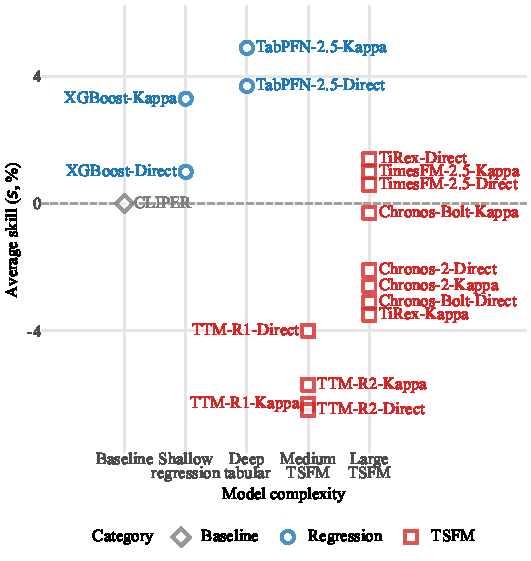
\includegraphics[scale=1]{skill_efficiency.pdf}
\caption{Schematic plot of model skill versus complexity.}
\label{fig:skille}
\end{figure}


\subsection{Performance under different sky conditions}
To investigate the performance of various forecasting models across different atmospheric states, I evaluate their performance by partitioning the dataset into three mutually exclusive sky conditions, namely, clear, cloudy, and overcast. This categorization is essential because irradiance predictability is not uniformly distributed; while clear-sky conditions offer deterministic predictability, the intermediate and overcast regimes introduce stochastic transients and diffuse-dominant scattering that challenge the representation capacity of foundation models.

The classification is implemented using the clearness index ($\epsilon$), as described by \citet{PEREZ1990271}, which is calculated as:
\begin{equation}
    \epsilon = \frac{(B_n + D_h)/D_h + 1.041 Z^3}{1 + 1.041 Z^3}
\end{equation}
where $B_n$ and $D_h$ are the BNI and DHI, the zenith angle $Z$ is in radians. This index captures the sky's optical state by analyzing the relationship between the diffuse and beam components of irradiance. Once the clearness index is computed for each 15-min timestamp, observations are assigned to a sky state based on the following $\epsilon$ ranges: overcast ($1 \le \epsilon \le 1.065$), cloudy ($1.065 < \epsilon \le 4.5$), and clear ($\epsilon > 4.5$). To ensure high-quality signals, I restrict this classification to daytime observations where $Z < 85^{\circ}$ and $G_h > 10 \text{ W/m}^2$.

To examine the performance, a conditional skill bar chart (see Fig.~\ref{fig:skillc}) is generated to show the average forecast skill ($s$) relative to the CLIPER baseline for each sky state. This highlights the ``efficiency gap'' by revealing which models fail to provide value during volatile intermediate conditions. In Fig.~\ref{fig:skillc}, data from all stations are lumped together, and for visual brevity, only the results from the two-step configuration of the models are displayed. The resulting performance breakdown confirms that the ``efficiency gap'' is most acute during cloudy conditions. For GHI, the regression-based TabPFN-2.5-Kappa and XGBoost-Kappa exhibit the highest resilience, yielding skill scores of 7.25\% and 6.77\%, respectively. In stark contrast, large-scale TSFMs like Chronos-2-Kappa ($-$1.63\%) and TiRex-Kappa ($-$1.92\%) fail to outperform CLIPER in this regime. This suggests that while foundation models possess high representation capacity, they struggle with the variability inherent in broken-cloud states that might be more effectively captured by structured regression. However, the foundation models demonstrate significant strength in the clear regime, where Chronos-2-Kappa (22.09\%) and TimesFM-2.5-Kappa (14.68\%) significantly outperform the tabular baselines. 

\begin{figure}[!ht]
\centering
\includegraphics[scale=1]{sky_condition_skill.pdf}
\caption{Comparative forecast skill ($s$) across three sky condition regimes for GHI and BNI.}
\label{fig:skillc}
\end{figure}

Interestingly, a reverse trend appears in the overcast BNI regime. While almost all models yield negative skill for GHI under overcast skies, TSFMs such as TiRex-Kappa (15.94\%) and TimesFM-2.5-Kappa (15.83\%) show high skill for the beam component. This suggests these models are particularly adept at identifying prolonged extinction events and maintaining a zero-beam forecast, whereas the persistence-climatology baseline likely suffers from lagged transitions at the overcast boundary. Overall, TabPFN-2.5-Kappa remains the most balanced architecture, maintaining positive and robust skill across both GHI and BNI in the variable cloudy regime where most other foundation models fail. 

\subsection{Discussion 1: Persistence hurdle}
A fundamental challenge in time series forecasting is the presence of a phase lag effect often referred to as the ``persistence hurdle.'' Particularly in stochastic time series where the sampling interval is short, such as the 15-min resolution utilized in this study, the immediate past observation ($x_t$) typically possesses the highest mutual information with the subsequent state ($x_{t+1}$). This high degree of temporal autocorrelation creates a statistical trap for supervised learning and foundation models alike: When the underlying physical drivers for a sudden change are not explicitly captured in the input features, the model minimizes the loss function by defaulting to a persistence-weighted forecast. Consequently, during transient atmospheric events such as the rapid onset of cloud cover, the forecast value $\hat{x}_{t+1}$ tends to shadow the previous observation $x_t$, resulting in a forecast that appears to be a delayed version of the ground truth, lagging by exactly one time step. 

This behavior is elucidated in Fig.~\ref{fig:dra}, which presents the time-series forecasts alongside the ground-truth observations for two contrasting representative days. Under clear-sky conditions, as exemplified by 2024-06-30, the clear-sky index ($\kappa$) remains approximately unity, allowing both supervised baselines and foundation models to track the deterministic solar trajectory with high precision. In this regime, the primary source of error is minimized as long as the clear-sky normalization is correctly applied during post-processing to reconstruct the irradiance profiles. Conversely, the period of 2024-12-22 illustrates a volatile, cloudy regime where the stochastic nature of the atmosphere dominates. During these intervals, all evaluated models---regardless of their architectural complexity or context length---fail to anticipate the high-frequency fluctuations in irradiance. This visualization demonstrates the persistence hurdle in a real-world context; because the models lack exogenous spatial awareness of incoming cloud structures, they are forced to react to changes only after they are registered by the local sensor. Consequently, the forecast transients appear as temporally shifted replicas of the observations, effectively hitting a predictability ceiling where the 1-step-ahead prediction is mathematically tethered to the most recent known state.

\begin{figure}
\centering
\includegraphics[scale=1]{dra_example.pdf}
\caption{Comparative GHI and BNI time-series for clear-sky (top) and cloudy (bottom) conditions. The latter highlights the severe persistence hurdle, characterized by a distinct temporal phase lag in model response.}
\label{fig:dra}
\end{figure}

This lagging behavior can be interpreted as a predictability ceiling inherent to univariate sequences. Formally, the 1-step-ahead forecast $\hat{x}_{t+1}$ is modeled as a function of its historical context:
\begin{equation}
\hat{x}_{t+1} = f(x_t, x_{t-1}, \dots, x_{t-C}, \mathbf{z}_t, \dots, \mathbf{z}_{t-C})
\end{equation}
where $C$ denotes the context length for foundation models or the length of historical data utilized for conventional models, and $\mathbf{z}$ represents exogenous temporal features. The philosophical deficiency of this extrapolative approach resides in the fact that $x_t$ typically contributes most to the forecast, forcing the transient of $\hat{x}_{t+1}$ to resemble the most recent observation. In summary, sophisticated foundation models like Chronos, TimesFM, or TiRex, which leverage vast context lengths ($C \in \{512, 1024\}$), remain fundamentally constrained by the persistence hurdle during volatile transient periods, despite their ability to improve the representation of the steady-state regime.

\subsection{Discussion 2: Forecast combination and oracle selection}
Forecast combination, also known as ensemble forecasting, is a well-known strategy to improve performance when multiple models are available. The core idea behind forecast combination is the ``wisdom of the crowd,'' where the over- and under-forecasts of various members cancel each other out, resulting in overall superior accuracy. To investigate the potential for such synergistic improvements in the current context, I evaluate three ensemble strategies alongside an oracle selector. The ensembles are categorized into a regression group (XGBoost and TabPFN), a TSFM group (the six foundation models), and an ensemble encompassing all eight models. The oracle represents a theoretical ``upper bound'' of performance, where the model with the lowest absolute error is perfectly selected for each 15-min interval.

\begin{table}
\centering
\footnotesize
\caption{RMSEs for GHI and BNI after various forecast combinations.}
\label{tb:combination}
\begin{tabular}{lrrrrrrrr}
\toprule
 & BON & DRA & FPK & GWN & PSU & SXF & TBL & Average \\
\midrule
& \multicolumn{8}{c}{GHI}\\
Regression & 69.9 (18.3) & 56.3 (10.9) & 70.6 (19.6) & 76.7 (19.0) & 82.7 (23.6) & 67.9 (18.6) & 89.5 (21.1) & 74.0 (18.5) \\
TSFMs & 72.9 (19.1) & 59.9 (11.6) & 73.7 (20.5) & 80.8 (20.1) & 86.4 (24.7) & 71.4 (19.6) & 94.4 (22.2) & 77.8 (19.5) \\
All & 69.5 (18.2) & 56.5 (11.0) & 70.6 (19.7) & 76.6 (19.0) & 82.5 (23.6) & 67.9 (18.6) & 89.7 (21.1) & 74.0 (18.5) \\
Oracle & \textbf{60.8 (15.9)} & \textbf{49.7 (9.6)} & \textbf{62.7 (17.5)} & \textbf{66.9 (16.6)} & \textbf{71.4 (20.4)} & \textbf{59.7 (16.4)} & \textbf{78.9 (18.6)} & \textbf{64.9 (16.2)} \\
\midrule
& \multicolumn{8}{c}{BNI}\\
Regression & 117.5 (29.5) & 104.9 (15.2) & 124.2 (30.1) & 111.1 (26.6) & 125.9 (36.7) & 115.8 (28.6) & 145.6 (28.4) & 121.3 (26.7) \\
TSFMs & 124.4 (31.3) & 112.6 (16.3) & 131.4 (31.8) & 118.4 (28.4) & 134.1 (39.1) & 124.1 (30.7) & 155.0 (30.2) & 129.2 (28.4) \\
All & 117.6 (29.6) & 105.0 (15.2) & 124.2 (30.1) & 111.2 (26.7) & 125.8 (36.7) & 116.4 (28.8) & 146.0 (28.5) & 121.5 (26.7) \\
Oracle & \textbf{102.9 (25.9)} & \textbf{90.2 (13.0)} & \textbf{108.5 (26.3)} & \textbf{96.3 (23.1)} & \textbf{108.0 (31.5)} & \textbf{102.3 (25.3)} & \textbf{126.7 (24.7)} & \textbf{105.5 (23.2)} \\
\bottomrule
\end{tabular}
\end{table}

Table~\ref{tb:combination} tabulates the RMSEs for both GHI and BNI across various combination strategies. The results indicate that simply increasing the number of ensemble members does not necessarily lead to superior performance. More specifically, while the overall best non-oracle performance occurs when all models enter the ensemble, the resulting RMSE remains statistically indistinguishable from the previous best-performing individual model, TabPFN, as shown in Tables~\ref{tb:RMSEGh} and \ref{tb:RMSEBn}. This outcome directly contrasts with previous findings in solar forecasting, where forecast combination almost universally leads to superior performance \citep[e.g.,][]{zhang2026, ZHANG2022111768}. Nevertheless, the regression ensemble consistently outperforms the TSFM group, achieving an average GHI nRMSE of 18.5\% compared to the 19.5\% yielded by the TSFMs, further suggesting the predictive superiority of the former.

The oracle analysis reveals the limitations inherent in the existing model pool. Even with a theoretical ``perfect'' selector that identifies the best forecast for every interval, the performance ceiling remains surprisingly high, with an nRMSE of 16.2\% for GHI and 23.2\% for DNI. At a site-specific level, such as PSU, even the oracle cannot achieve better than a 20.4\% nRMSE. This suggests that the primary barrier to leaping the persistence hurdle is not merely the difficulty of model selection, but a fundamental lack of accurate predictive trajectories within the current architectures---whether regression or foundation-based---for complex atmospheric states. Consequently, even an ideal integration of these models remains insufficient for the high-precision forecasting required by grid integration.

\section{Conclusion}
This study provides a comprehensive evaluation of the latest time-series foundation models (TSFMs) for univariate solar irradiance forecasting, specifically investigating whether zero-shot representations can overcome the ubiquitous persistence hurdle in the 15-min-ahead setting required for grid integration. By benchmarking state-of-the-art models released in the past two years across seven geographically diverse sites, several critical conclusions are drawn regarding the current state of foundation models in highly variable physical contexts.
\begin{itemize}
    \item The efficiency gap: A profound gap exists between general-purpose TSFMs and structured regression models. While large-scale models like Chronos and TimesFM possess superior representation capacity, they frequently fail to provide positive forecast skill relative to the CLIPER reference, primarily due to an inability to overcome the persistence-induced phase lag.
    \item Superiority of structured priors: The regression-based TabPFN emerges as the best-performing architecture, consistently achieving a 5\% forecast skill for both GHI and BNI. This success underscores the importance of explicit physical feature engineering, such as solar geometry or temporal cycles, over pure sequence modeling for high-frequency solar transients.
    \item The persistence ceiling: The oracle analysis demonstrates that even with ``perfect'' model selection, a theoretical performance ceiling persists, with nRMSE values remaining as high as 16.2\% for GHI. This suggests that the primary barrier to high-precision forecasting is not just model selection, but a fundamental deficiency in current architectures' ability to generate accurate predictive trajectories for complex atmospheric states.
\end{itemize}
In summary, while foundation models offer a promising zero-shot alternative to data-hungry traditional methods, their current iterations are not yet a panacea for the stochastic complexities of solar irradiance. Future research should focus on hybridizing the ``temporal grammar'' of TSFMs with the physical vision provided by sky cameras to finally leap the persistence hurdle in operational renewable energy integration.


\section*{Acknowledgements}
This work is supported by the National Natural Science Foundation of China (project no. 42375192).

\section*{Data availability}
This paper is reproducible. Data and code can be accessed via \url{https://gitee.com/dazhiyang/tsfm-solar} repository on Gitee under MIT license.

% \appendix
% \section{Data availability}
% \label{App:Sup}
% The data used for this paper will be uploaded to the official website of the Baseline Surface Radiation Network (BSRN), under the station abbreviation QIQ, station number 94.

%\section*{Acknowledgments}
%European Centre for Medium-range Weather Forecast (ECMWF) operational forecast and analysis data used in this study were downloaded from the ECMWF Meteorological Archival and Retrieval System (MARS) in 2022.  Access to the ECMWF archived data was provided by ECMWF's Data Services. Special thanks go to Emma Pidduck, Ruth Coughlan, and Ilaria Parodi from the ECMWF's Data Services team, for their swift communication regarding data access.



\bibliographystyle{elsarticle-num-names}
\bibliography{MyBibFile}


\end{document}


